\documentclass[10pt, a4paper, twosize]{article}
%\documentclass[12pt, a4paper, twoside]{book}

\usepackage{helvet}
\usepackage{hyperref}
\usepackage{graphicx}
\usepackage{listings}
\usepackage{textcomp}
\usepackage[
	a4paper,
	outer=2cm,
	inner=4cm,
	top=2cm,
	bottom=2cm
]{geometry}
\usepackage{float}
\usepackage{tabularx}
\usepackage[disable]{todonotes}
\usepackage{color, soul}
\usepackage{amsmath}
\usepackage{algorithmicx}
\usepackage[noend]{algpseudocode}
\usepackage{algorithm}
\usepackage{framed}
\usepackage{subcaption}
\usepackage{titlepic}
\usepackage{fancyhdr}
\usepackage[simplified]{styles/pgf-umlcd}
\usepackage{shorttoc}
\usepackage{url}
\usepackage{paralist}
\usepackage{multicol}

\definecolor{grey}{rgb}{0.9, 0.9, 0.9}
\definecolor{dkgreen}{rgb}{0,0.6,0}
\definecolor{dkred}{rgb}{0.6,0,0.0}

\lstdefinestyle{DOS}
{
    backgroundcolor=\color{black},
    basicstyle=\scriptsize\color{white}\ttfamily,
    stringstyle=\color{white},
    keywords={}
}

\lstdefinestyle{makefile}
{
    numberblanklines=false,
    language=make,
    tabsize=4,
    keywordstyle=\color{red},
    identifierstyle= %plain identifiers for make
}

\lstset{
  language=Java,                % the language of the code
  basicstyle=\footnotesize\ttfamily,
  numbers=left,                   % where to put the line-numbers
  stepnumber=1,                   % the step between two line-numbers. If it's 1, each line
  numbersep=5pt,                  % how far the line-numbers are from the code
  backgroundcolor=\color{white},      % choose the background color. You must add \usepackage{color}
  showspaces=false,               % show spaces adding particular underscores
  showstringspaces=false,         % underline spaces within strings
  showtabs=false,                 % show tabs within strings adding particular underscores
  frame=single,                   % adds a frame around the code
  rulecolor=\color{black},        % if not set, the frame-color may be changed on line-breaks within not-black text (e.g. comments (green here))
  tabsize=2,                      % sets default tabsize to 2 spaces
  captionpos=b,                   % sets the caption-position to bottom
  breaklines=true,                % sets automatic line breaking
  breakatwhitespace=false,        % sets if automatic breaks should only happen at whitespace
  keywordstyle=\color{blue},          % keyword style
  commentstyle=\color{dkgreen},       % comment style
  stringstyle=\color{dkred},         % string literal style
  columns=fixed,
  extendedchars=true,
  frame=single,
}

%\renewcommand{\chaptername}{Topic}

% New definitions
\algnewcommand\algorithmicswitch{\textbf{switch}}
\algnewcommand\algorithmiccase{\textbf{case}}
\algnewcommand\algorithmicassert{\texttt{assert}}
\algnewcommand\Assert[1]{\State \algorithmicassert(#1)}%
% New "environments"
\algdef{SE}[SWITCH]{Switch}{EndSwitch}[1]{\algorithmicswitch\ #1\ \algorithmicdo}{\algorithmicend\ \algorithmicswitch}%
\algdef{SE}[CASE]{Case}{EndCase}[1]{\algorithmiccase\ #1}{\algorithmicend\ \algorithmiccase}%
\algtext*{EndSwitch}%
\algtext*{EndCase}%

\pagestyle{fancy}
\fancyhf{}
\fancyhead[RO, LE]{\small \rightmark}
\fancyfoot[RO, LE]{\small \thepage}

\begin{document}

%\frontmatter

\begin{titlepage}
\vspace*{5cm}
\begin{center}

\includegraphics[width=.5\textwidth]{images/EdNapUniLogoCMYK}~\\[1cm]

\textsc{\Large Edinburgh Napier University}\\[1.5cm]

\textsc{\LARGE \bfseries SET08101 Web Tech}\\[0.5cm]

\hrulefill \\[0.4cm]
{\huge \bfseries Lab 8 - Webapps Using Node.JS) \\[0.4cm] }
\hrulefill \\[1.5cm]

\begin{minipage}{0.4\textwidth}
\begin{flushleft} \large
\textbf{Dr Simon Wells} \\
\end{flushleft}
\end{minipage}

\vfill

\end{center}
\end{titlepage}

%\shorttoc{Overview}{0}

%\setcounter{tocdepth}{2}
%\cleardoublepage
%\tableofcontents
%\listoffigures
%\listofalgorithms
%\addtocontents{toc}{~\hfill\textbf{Page}\par}

%\mainmatter

%\input{sections/labs/04_ui}

\section{Aims}
\paragraph{} Our aim this week is to use JavaScript on the server side to generate our website from code. In previous weeks we've assumed that we know all the things that are going to happen, and everything that need to be displayed, at design time. However, quite often we will want to generate our HTML, perhaps based upon whether the user is logged in, or based upon a query supplied by the user. Over the next couple of weeks we'll add more features to this approach, such as using a datastore to hold the data for our web-app or using a RESTful approach to design our site. Before then, we need to see how to use JS to generate our website.

\paragraph{} At the end of the practical portion of this topic you will:

\begin{itemize}
\item Install the Express framework \& related supplementary Node packages
\item Route HTTP requests in Node using the Express framework
\item Generate an Express web-app and start using the Pug templating engine
\end{itemize}


%\begin{framed}
%{\bf{NOTICE:}  }
%\end{framed}


\section{Activities}

\subsection{The Express Framework}
\paragraph{} Express is a simple, minimal, and flexible web application framework for Node. It can be used to rapidly build robust and scalable web and mobile applications.

\paragraph{} First we need to install the Express framework so that Node can use it. We'll use npm for that just like last week\footnote{If you haven't completed the introduction to Node from last week then do that first otherwise the rest of this lab is just going to be increasingly confusing.}. So navigate to the folder that holds node.exe then, using he Windows command line do:

\begin{lstlisting}[style=DOS]
    > npm install express --save
\end{lstlisting}

\paragraph{} After a few moments you should have the express framework and we can start using it. Create a folder, ``helloexpress'' then add a file called helloexpress.js into it. Edit helloexpress.js as follows:

\begin{lstlisting}
var express = require('express');
var app = express();

app.get('/', function (req, res) {
   res.send('Hello Express');
})

var server = app.listen(5000, "127.0.0.1", function () {
   var host = server.address().address
   var port = server.address().port
   
   console.log("Listening on http://%s:%s", host, port)
})
\end{lstlisting}

\paragraph{}

\paragraph{} We can now run that simple express web app as follows:

\begin{lstlisting}[style=DOS]
    > node helloexpress.js
    Listening on http://127.0.0.1:5000
\end{lstlisting}

\paragraph{} Note that the output from running this should be a message telling us that the web-app is running and suggesting a URL that it is available at. Note that 127.0.0.1 is an IP address that points to your local machine. If it doesn't work on your machine then you can also try \url{http://localhost:5000} and \url{http://0.0.0.0:5000} as there canbe some variation between machines, operating systems, and browser versions. All three addresses all basically mean the local machine however and are different ways of expressing the same concept.

\begin{figure}[H]
%\centering
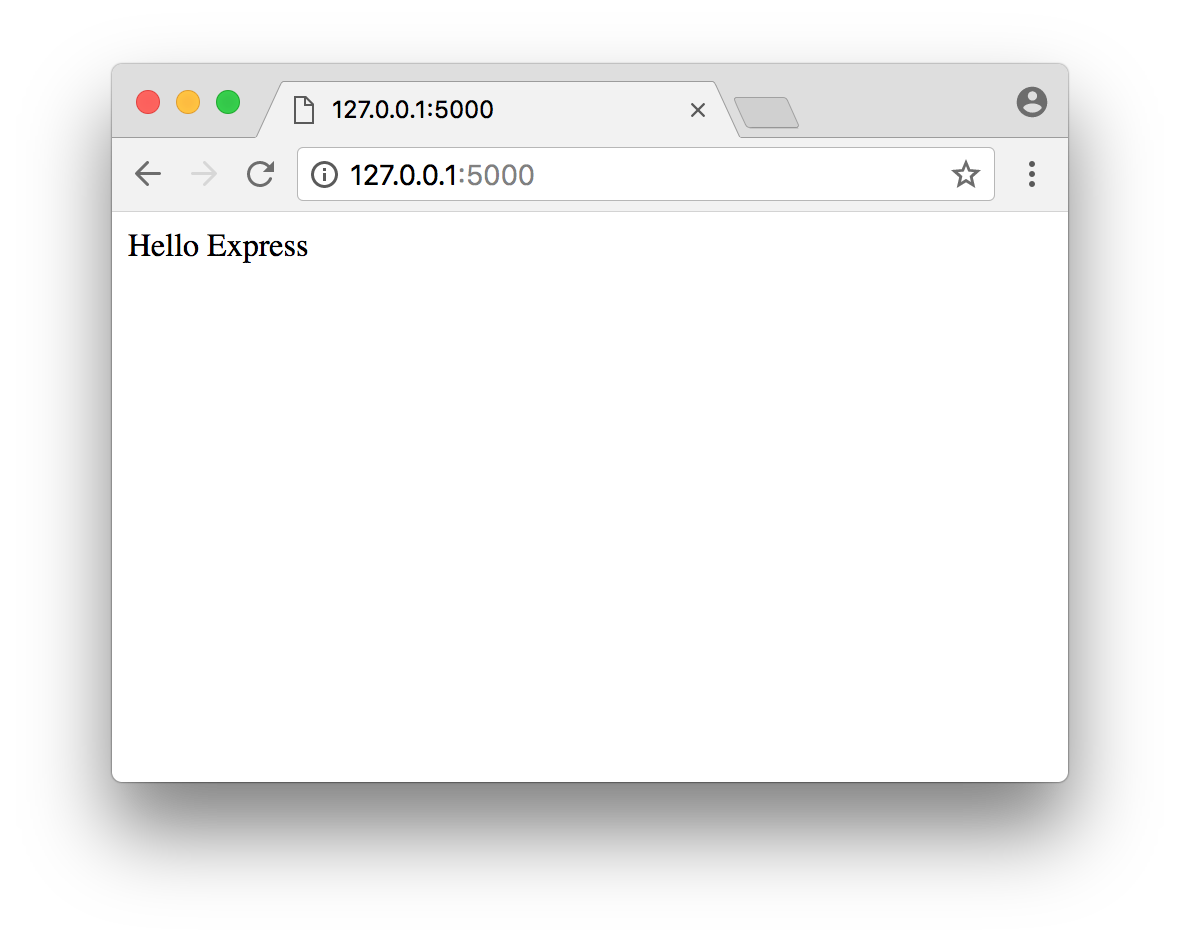
\includegraphics[width=0.85\textwidth]{images/express_helloexpress}
\caption{The output from the helloexpress.js web app}
\label{fig:express_helloexpress}
\end{figure}


\subsection{Routing in Express}
\paragraph{} Really all a web-app has to do is route messages around, for example, handle an incoming message to a given url and return the correct result (usually some HTML) so nearly all web-app frameworks are built around the concept of routing and Express is no different. What are the message that Express routes around? Basically they are objects reprepresenting core concepts of HTTP; requests and responses. Our web-app will recieve a request and return the correct response. Until now this has been straightforward because the correct response for a static web-server when it receives a request is to send back the resource that was requested. However with web-apps we intend to add some dynamic behaviour rather than merely returning static resources.

\paragraph{} Express web-apps use \emph{callback functions} to implement routing. The parameters passed to the callback functions are \emph{request} and \emph{response} obejects. This fragment gives you some indication of the structure of an express callback (we'll use it in earnest over the next few examples):

\begin{lstlisting}
app.get('/', function (req, res) {
   // We would include what the function does here
})
\end{lstlisting}

\paragraph{} Notice that there are \emph{req}uest and \emph{res}ponse objects passed to the function as parameters. These directlt represent the incoming HTTP request and outgoing HTTP response, respectively. Something else to notice is that we can almost read the first line as follows" ``the app object has a get method for the root (/) route that takes a request object, does some stuff and finally returns a response object''. We can also interact with those req and res objects from code, for example we can print them to find out information about the incoming request or what information is stored by default in the response. We can of course also manipulate the response object. In fact, we've already seen a working example of a callback function in our helloexpress example earlier, e.g.

\begin{lstlisting}
app.get('/', function (req, res) {
   res.send('Hello Express');
})
\end{lstlisting}

\paragraph{} Note that in order to get ``Hello Express'' to be displayed in the browser we called the send() method of the response object. We can interact with the response object in a number of interesting ways.

\paragraph{} For the moment though, let's consider one of the primary aspects of HTTP, particularly in relation to REST. That is, HTTP verbs. The different ways that a client can interact with an HTTP resource are primarily described by HTTP verbs. We've already seenand probably used thousands of time, the HTTP GET verb. This is the verb that is sent by default when a browser or other client interacts with an HTTP resource. Note that for the moment we'll consider an HTTP resource to be some data located at a given web address. We can interact with that resource at the given address in a whole bunch of different ways. For the moment let's consider the localhost ``/'' resource. Without doing anything cleve in JS or anything else, we can use different HTTP verbs to cause the server to do different things in relation to the resource just by calling the resource in different ways. For example:


\begin{lstlisting}
var express = require('express');
var app = express();

app.get('/', function (req, res) {
   res.send('A GET request to the root resource');
})

app.post('/', function (req, res) {
   res.send('A POST request to the root resource');
})

app.head('/', function (req, res) {
   res.send('A HEAD request to the root resource');
})

var server = app.listen(5000, "127.0.0.1", function () {
   var host = server.address().address
   var port = server.address().port
   
   console.log("Listening on http://%s:%s", host, port)
})
\end{lstlisting}

\paragraph{} We have a small problem though. Our browser doesn't, by default, allow us to easily call routes using verbs other than GET. We could make a POST request if there was an HTML button to press, but other than that we are a bit stuck. We can use others verbs from JS though, and there are lots of tools to let us use those verbs, but browsers aren't one of them. We should consider why this is. Mostly it is because the web, as supported by HTTP, is about more than just accessing data from a web browser. There are many web clients that aren't browsers, for example, mobile applications, really anything that can consume an HTTP API.

\paragraph{} One such tool is cURL, a command line application that is installed by default on many Linux and Mac machines and which is an easy download away for Windows users. Download the latest zip file from \url{https://curl.haxx.se/download.html} then unzip it somewhere useful. Note that the archives at the top of that page refer to the source code for the program. You should navigate down to the ``Win32 Generic'' section and download the latest zip from there\footnote{I downloaded the following when testing things out recently: \url{https://dl.uxnr.de/build/curl/curl_winssl_msys2_mingw32_stc/curl-7.58.0/curl-7.58.0.zip}}. You'll then need to navigate to that location using the Windows command line and find curl.exe which was located in the src folder on the build that I downloaded.

\paragraph{} We can now use cURL to call our various routes, for example, calling the GET route:

\begin{lstlisting}[style=DOS]
    > curl.exe http://localhost:5000
    A GET request to the root resource
\end{lstlisting}

\paragraph{} Notice how the output is similar to what we would get in the browser. We can now also call the POST route:

\begin{lstlisting}[style=DOS]
    > curl.exe http://localhost:5000 -X POST
    A POST request to the root resource
\end{lstlisting}

\paragraph{} This time the output is different because we couldn't issue a POST request directly from the browser without implementing a button on a web page to issue the POST. However, cURL lets us issue the request directly. Let's try the PUT verb:


\begin{lstlisting}[style=DOS]
    > curl.exe http://localhost:5000 -X PUT
    <!DOCTYPE html>
    <html lang="en">
    <head>
    <meta charset="utf-8"
    <title>ERROR</title>
    </head>
    <body>
    <pre>Cannot PUT /</pre>
    </body>
    </html>
\end{lstlisting}

\paragraph{} Ahhh. This is different. We got an error. This is because we haven't implemented a handler for PUT requests to this route. Instead, when our node app receives the request an error page is automatically generated in HTML.

\paragraph{} Finally, let's call that HEAD route and see what happens:

\begin{lstlisting}[style=DOS]
    > curl.exe http://localhost:5000 --head
    HTTP/1.1 200 OK
    X-Powered-By: Express
    Content-Type: text/html; charset=utf-8
    Content-Length: 34
    ETag: W/"22-4d0H1eyiftrrcLVM4PJK+kdQ6Nc"
    Date: Mon, 26 Feb 2018 17:15:03 GMT
    Connection: keep-alive

\end{lstlisting}

\paragraph{} Hmmmm. That's different again. Firstly, we had to call this verb using the --head argument instead of using -X head as we would for PUT, POST, etc. Additionally, we on't see the actual content of the response from the / route when we use the HEAD command. Instead we just get the header information. That's the point, HEAD is really useful for getting the information that the server will send back from a route but ignoring the actual body of the document, i.e. the HTML document. 

\paragraph{} Express supports a whole bunch of routing methods that correspond to HTTP verbs, for example:

\begin{multicols}{3}
\begin{itemize}
\item checkout
\item copy
\item delete
\item get
\item head
\item lock
\item merge
\item mkactivity
\item mkcol
\item move
\item m-search
\item notify
\item options
\item patch
\item post
\item purge
\item put
\item report
\item search
\item subscribe
\item trace
\item unlock
\item unsubscribe
\end{itemize}
\end{multicols}

\paragraph{} This is an opportunity to do some background reading. First have a look at tthe Express documentation\footnote{\url{https://expressjs.com/en/api.html}} then perhaps investigate HTTP verbs; the Mozzila developer documentation is a good place to start\footnote{\url{https://developer.mozilla.org/en-US/docs/Web/HTTP/Methods}}.

\subsection{Raw HTML from Express}
\paragraph{} So far we've only returned plain text from Express. What we probably want to do is to respond with an HTML document. We can do that in code, or using a templating library. Let's start with generating some raw HTML in our response:

\begin{lstlisting}
var express = require('express');
var app = express();

app.get('/', function (req, res) {
    res.set('Content-Type', 'text/html');
    res.send(new Buffer('<h1>The root route</h1>'));
   })

app.get('/hello', function (req, res) {
    res.set('Content-Type', 'text/html');
    res.send(new Buffer('<h2>The hello route</h2>'));
   })

app.get('/goodbye', function (req, res) {
    res.set('Content-Type', 'text/html');
    res.send(new Buffer('<p>The <b>goodbye</b> route</p>'));
    })


var server = app.listen(5000, "127.0.0.1", function () {
   var host = server.address().address
   var port = server.address().port
   
   console.log("Listening on http://%s:%s", host, port)
})
\end{lstlisting}

\paragraph{} We'll revist this later because we can use a similar approach to return JSON instead of HTML. That said, Express has a much better way to deal with HTML, using templates.

\subsection{Using Templates from Express}
\paragraph{} Express uses template engines to control the generation of HTML so that we don't have to do everything from scratch. Instead we create templates that Express processes to generate the HTML documents that are returned to the client. 

\paragraph{} To use templates with Express we need to install some extra packages using NPM. First Pug which is a templating engine\footnote{The Pug project is here: \url{https://pugjs.org/}}:

\begin{lstlisting}[style=DOS]
    > npm install pug --save
\end{lstlisting}

\paragraph{} We also need the express-generator package which gives us a way to generate the skeleton of an express web-app:

\begin{lstlisting}[style=DOS]
    > npm install express-generator -g
\end{lstlisting}

\paragraph{} Now we can use the express generator to create our skeleton. We'll also specify to use pug and give the name of our new app as helloapp

\begin{lstlisting}[style=DOS]
    > express --view=pug helloapp
\end{lstlisting}

\paragraph{} This will generate a structure containing bin, public, routes, and views folders as well as an app.js file and a package.json file. Explore the various folders and files. Notice that views contains a number of files that end in `.pug' which are the tempaltes for your HTML pages. 

\begin{figure}[H]
%\centering
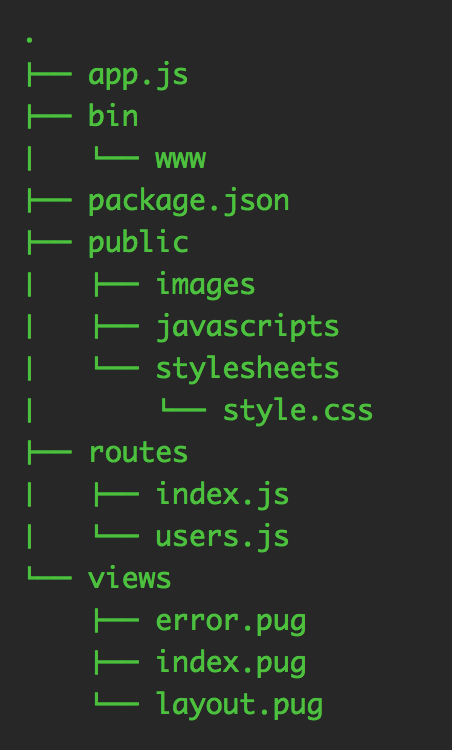
\includegraphics[width=0.65\textwidth]{images/express_structure}
\caption{The structure of the Express web app generated by express-generator.}
\label{fig:express_structure}
\end{figure}


\paragraph{} Once a skeleton is generated we can use npm to install all the Node modules that our new express app needs, e.g.

\begin{lstlisting}[style=DOS]
    > npm install
\end{lstlisting}

\paragraph{} This will cause a folder called node\_modules to be created and a bunch of standard packages to be installed into it. You should be getting the idea now that Node likes to break things down into lots of smaller packages then give you tools to help manage them all.

\paragraph{} This should be enough set up to enable us to get a basic express app running. One last small thing to do if we're on a JKCC lab machine is to alter the port number that our app will run on. The default is 3000 and we have 5000 reserved for use on this module. So open the file called www in the folder called bin and change the following line:

\begin{lstlisting}
var port = normalizePort(process.env.PORT || '3000');
\end{lstlisting}

to:

\begin{lstlisting}
var port = normalizePort(process.env.PORT || '5000');
\end{lstlisting}

\paragraph{} Now let's run our app\footnote{If you're on Mac or Linux then do this instead: \$ DEBUG=myapp:* npm start:}:

\begin{lstlisting}[style=DOS]
    > set DEBUG=myapp:* & npm start
\end{lstlisting}

\paragraph{} We should now be able to access our app in our browser by visiting \url{localhost:3000}.

\paragraph{} To add additional routes to our web-app, we merely add them to the routes/index.js file. This should look familiar because it's similar to what we were editing earlier when we were using Node without the express framework. This is index.js:

\begin{lstlisting}
var express = require('express');
var router = express.Router();

/* GET home page. */
router.get('/', function(req, res, next) {
  res.render('index', { title: 'Express' });
});

module.exports = router;
\end{lstlisting}

\paragraph{} We can add whichever routes we want to \emph{routes/index.js} like so:

\begin{lstlisting}
var express = require('express');
var router = express.Router();

/* GET home page. */
router.get('/', function(req, res, next) {
  res.render('index', { title: 'Express' });
});

router.get('/hello', function(req, res, next) {
  res.render('index', { title: 'The Hello Route' });
});

module.exports = router;
\end{lstlisting}

\paragraph{} We can also add extra templates as required into the views folder. These all use the Pug language instead of HTML. For example, the template used by both the index and hello routes above is the index.pug file which looks like this:

\begin{lstlisting}
extends layout

block content
  h1= title
  p Welcome to #{title}
\end{lstlisting}

\paragraph{} Notice that both routes are using the same template, the idea is to capture the common aspects of the different HTML pages that will make up our site. This way we can have a small number of templates, but perhaps hundreds or even thousands of pages can use the same template. By suppling different data to the template from the route function we get the tempalte to be completed in different ways which leads to different HTML being generated and returned to the browser. For example, our root and hello functions in routes/index.js are passing different data to the template so that the title parameter is compelted differently. Using templates make it even more important to think about the layout of your site before you try to build it. A rough preliminary design will give your some idea of how many templates are needed and this number should, as a rule be much lower than your total number of HTML pages. If you have as many templates as HTML pages then you're doing it wrong.

\paragraph{} It's well worth exploring the Pug and Express documentation to get a better idea of what you can do with these powerful tools. A good exercise to try is to attempt to turn your cipher website into an Express app as you should already have a good idea of what you site should look like, what pages it needs, and which elements are common to multiple pages and can be extracted into templates.


\end{document}

%\begin{framed}
%\end{framed}


%\begin{lstlisting}
%\end{lstlisting}


%\begin{lstlisting}[style=DOS]
%\end{lstlisting}


%\begin{figure}[H]
%\centering
%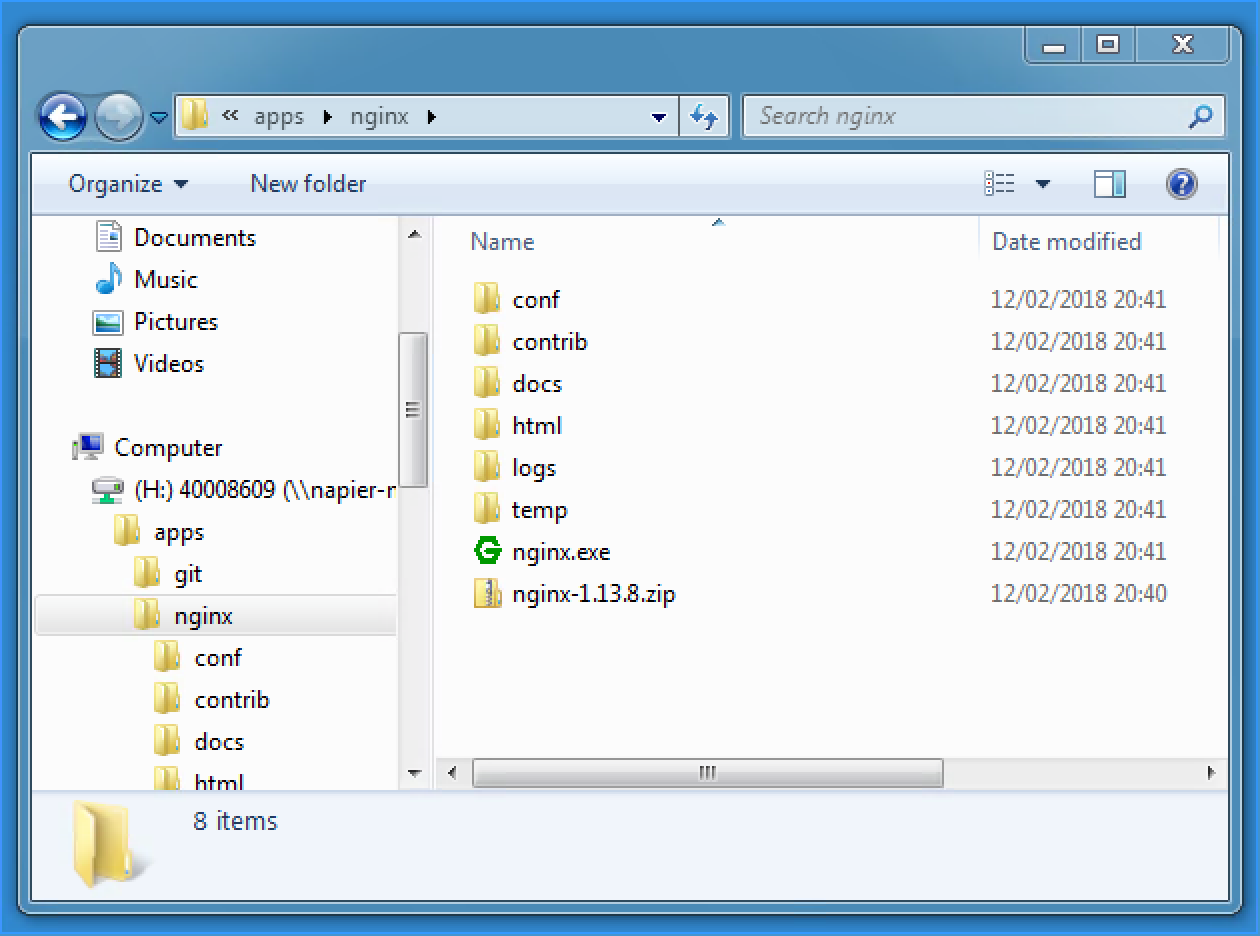
\includegraphics[width=0.85\textwidth]{images/nginx_exe}
%\caption{The nginx executable.}
%\label{fig:nginx_welcome}
%\end{figure}
